\documentclass[conference]{IEEEtran}
\IEEEoverridecommandlockouts
% The preceding line is only needed to identify funding in the first footnote. If that is unneeded, please comment it out.
\usepackage{cite}
\usepackage{amsmath,amssymb,amsfonts}
\usepackage{algorithmic}
\usepackage{graphicx}
\usepackage{textcomp}
\usepackage{xcolor}
\usepackage{float}

\pagestyle{plain}


\def\BibTeX{{\rm B\kern-.05em{\sc i\kern-.025em b}\kern-.08em
    T\kern-.1667em\lower.7ex\hbox{E}\kern-.125emX}}
\begin{document}

\title{Identifying Hate Speech Categories On Social Media\\
}

\author{\IEEEauthorblockN{Jack Ryan Cracknell}
\IEEEauthorblockA{\textit{School of Electronic Engineering and Computer Science} \\
\textit{Queen Mary University of London}\\
London \\
jcracknell123@gmail.com / EC20046@qmul.ac.uk}
}

\maketitle

\begin{abstract}
With the ever increasing popularity of social media within our society, there exists a growing amount of people using such platforms to cause harm. Through natural language processing models, it is possible to detect when a social media post contains hate speech. These models can be used to autonomously moderate sites and remove hateful or offensive messages. One issue with this approach is that it may be difficult for data to be collected by such models that show their effectiveness at removing various subgroups of hate speech. In this paper, a model will be created which aims to identify the specific type of hate speech that a message contains. Through this model, social media sites could collect data on which hate speech is most rampant, and make adjustments to their post moderation algorithms accordingly.
\end{abstract}

\begin{IEEEkeywords}
Social media, Hate speech
\end{IEEEkeywords}

\section{Introduction}
Hate speech has been defined as 'any communication that disparages a person or a group on the basis of some characteristics such as race, colour, ethnicity, gender, sexual orientation, nationality, religion, or other characteristics' \cite{b1}. \\
With the ever growing population of social media sites, there has been an explosion of posts that have been uploaded to them. Due to this, there has also been an increase in the amount of hateful activity online. Some of this hateful activity has been broadcast in real time on social media sites, such as the Christchurch shooting in 2019 \cite{b6}. Successfully identifying these hate speech messages through machine learning models aids in removing not only the messages themselves but also similar posts, stemming the amount of hate that can be spread. Having a state-of-the-art hate speech classification model may also increase the speed and accuracy at which social media sites can identify possible perpetrators of hateful actions in the real world, since many individuals who commit violent hate crimes have previously posted hate speech online \cite{b7} Furthermore, having the ability to classify hate speech posts into the most relevant subclass can give insight into what type of hate is most prevalent.\\
Before automatic natural language processing (NLP) models were introduced, websites would aim to block hate speech by having filters around specific words and phrases, but this is extremely time consuming. Word filters also scale poorly due to the quick evolution of language \cite{b2, b3}. Therefore an effective NLP model must be adaptable to new language and efficient in parsing through huge datasets. \\
There are various NLP methods for tackling hate speech online. Some classical approaches include Logistic regression, Support Vector Machines and Bayes models. In recent years, neural network models have become the industry standard state-of-the-art approach \cite{b4}, although in some cases, the results given by neural networks can be difficult to interpret \cite{b5}. \textbf{cite here to show that NNs would be difficult for this task due to a small dataset - which is why this project focuses on classical approaches to classification}

social media (using twitter data for this proj), Mention collecting multiple data sources together for a large range of different hate speech types.\\ Talk about some issues past papers (bias, unbalanced classes, different perceptions of hate speech) have come across and how they will be answered by my research

\section{Background and related work}
Related papers on hate speech detection, word filters, nlp models, find a paper on 'cyberbullying'
Background topics
specific NLP models and their background / papers they were developed on.

\subsection{Classification models}
\paragraph{\textbf{Logistic Regression}} This classifier is a supervised machine learning algorithm which predicts a target probability value between 0 and 1. This is achieved through the following equation.
\[y = \frac{\exp(\beta_{0} + \beta_{1} \text{data})}{1 + \exp(\beta_{0} + \beta_{1} \text{data})}\]
The data that will be used in this project will be preprocessed tweets, $\beta_{0}$ is the bias term and $\beta_{1}$ is the coefficient term for the input data. This coefficient term is learned from the training data. \textbf{possibly expand here}

For a binary classification task, \textit{y} will be the probability of the default class. The default class will be the tweet containing no hate speech. This is represented by the equation \[ P(Hate=False | Tweet) \]
\noindent
Where P $<$ 0.5, the sample will be classified as 0 - no hate\\
Where P $>$ 0.5, the sample will be classified as 1 - hate\\
\noindent
\\The methodology differs slightly when more than two classes are involved as logistic regression does not natively support multi-class classification. This new technique is named \textit{'one vs rest'} - hereby referred to as OvR splits the problem up into multiple binary classification tasks.\\
\begin{itemize}
  \item Binary Problem 1: Class1 vs [Class2, Class3, Class4]
  \item Binary Problem 2: Class2 vs [Class1, Class3, Class4]
  \item Binary Problem 3: Class3 vs [Class1, Class2, Class4]
  \item Binary Problem 4: Class4 vs [Class1, Class2, Class3]\\
\end{itemize}

OvR takes a single classifier per class, where samples classified as the current target class are represented as positive, and all other samples are negative\cite{b8}. Each classifier produces a confidence score. The predicted class label is chosen by the corresponding highest confidence model. OvR has some scalability issues that become apparent with very large class sets or slow models due to the need of creating a single model for each label, though these issues do not appear in this project.\\

\paragraph{\textbf{Support Vector Machine}} SVMs are a type of supervised learning algorithm that aims to predict a target class by separating data samples by a hyperplane. SVMs decide on the most optimal hyperplane by selecting that which has the largest distance from data samples on each side of the separator. \textit{'Support vectors'} refer to samples which are closest to the separating line. The position of these vectors changes the size of the margin depending on their location. These can be seen in figure \ref{fig:support_vectors},

\begin{figure}[h]
    \centering
    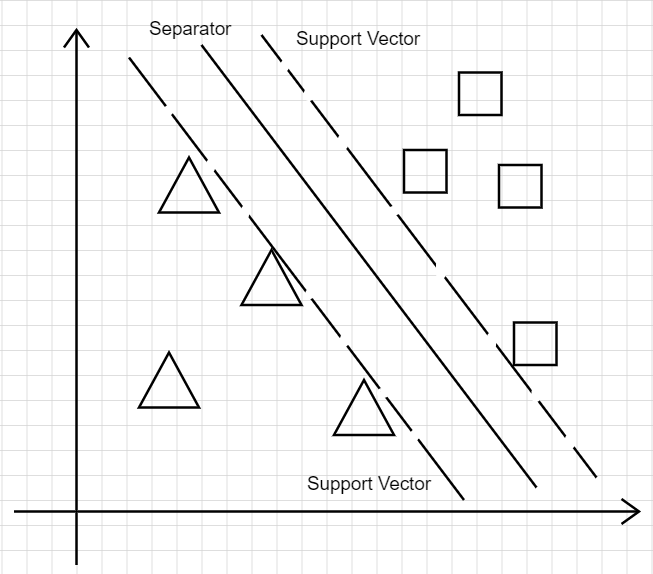
\includegraphics[width=0.35\textwidth]{Support_vectors.png}
    \caption{Example of a linear separator with support vectors}
    \label{fig:support_vectors}
\end{figure}

When more than two classes are introduced to an SVM, the classifier takes the same approach as logistic regression, utilising OvR. In this case, a separating margin will be drawn between the target class sample and the \textit{rest} of the dataset. The label with the corresponding highest confidence margin will be chosen as the prediction.\\

\paragraph{\textbf{Naive Bayes}}
Naive Bayes (namely GaussianNB which will be used in this project) is a supervised learning algorithm based on the \textit{Bayes' Theorem}

\[P(A|B) = \frac{P(A) \cdot P(B|A)}{P(B)}\]

In the above equation, P(A) is the probability of A occurring, P(B) is the probability of B occurring, P(A$|$B) is the probability of A given B has occurred and P(B$|$A) is the probability of B given A has occurred. This equation can also be written in context of this project.

\[P(Hate|Tweet) = \frac{P(Hate) \cdot P(Tweet|Hate)}{P(Tweet)}\]

Tweet contains a feature vector containing the preprocessed words in each tweet sample. In Naive Bayes, there is an assumption of independence between the data samples supplied, specifically, each word in the tweet would contribute independently to the class prediction. Using this independence assumption, we calculate the likelihood of a class label being predicted by the sum of the probabilities of observing each word in the tweet

\[P(Hate|word_1 ... word_n) = \] 
\[P(Hate) \cdot P(word_1|Hate)... P(word_n|Hate)\]

Bayes' models will calculate probabilities for all classes through these equations, making it well suited for both binary and multi-class problems.
The Bayes' classifier that has been used in this project is Gaussian Bayes' which adds the assumption that the continuous values associated with each class are in the form of a Gaussian distribution. The application of this is particularly interesting when the tweet text is vectorised.
\textbf{POSSIBLY PUT GAUSSIAN EQUATION IN HERE}

\subsection{Word embedding}
Word embeddings are a way to represent words in a text as a number or vector rather than their initial string format. The main idea which underpins word embeddings is that words that have similar meaning will be closer together in vector space. Many different vectorisers exist, though three have been chosen for this project.\\

\paragraph{\textbf{Count vectorisation}} This technique is simply word representation, a vector is built with size equal to the amount of unique words in the text. When a word appears in the corpus, it will be added to the vector representation matrix, if this word appears again, the count will be increased. Using this method on a large text corpus tends to make each count vector very sparse. Count vectors contain no information about the relation or similarity between words, the only information stored is whether the word appears or not. An example of a count vector is shown below.

\[Vocabulary = \{thanks; hello; for; reading; thanks\} \] 
Vector representation matrix:
\begin{table}[H]
\centering
\begin{tabular}{|l|l|l|l|}
\hline
thanks & hello & for & reading \\ \hline
2      &   0   &  0  &    0 \\ \hline
0      &   1   &  0  &    0 \\ \hline
0      &   0   &  1  &    0 \\ \hline
0      &   0   &  0  &    1 \\ \hline
\end{tabular}
\end{table}

If we then have a sentence in our dataset which consists of the text "reading for homework", the feature vector would have a size of 4 - the length of the vocabulary and have a 1 indices 2 and 3.
\[ [0, 0, 1, 1]\]

Given a much larger corpus vocabulary, it is evident that the count vector can see increasing amounts of sparsity. This is quite prevalent in the context of this project as the vocabulary of all words in the dataset is quite large in comparison with the average amount of words in a tweet.\\

\paragraph{\textbf{TFIDF}}
TFIDF is the acronym for Term Frequency Inverse Document Frequency. This is combination of two other statistical metrics.\\
\textbf{Term Frequency} - a count of how many instances of a word appear in total within a text. This is formally represented as:

\[ TF = \frac{Number\: of\: times\: a\: word\: appears\: in\: text}{total\: number\: of\: words\: in\: text}\]

\textbf{Inverse Document Frequency} - IDF is a metric that is concerned with weighting how much information a word in a text can give. Since IDF is an inverse fraction, it supplies a higher weighting for rarer terms whilst giving a lower weight to more frequent terms. Formally:

\[ IDF = log \frac{total \: number \: of \: texts \: in \: a \: corpus}{number \:
of \: texts \: where \: word \: appears}\]

Finally, these two terms are combined to calculate TFIDF:

\[ TFIDF = TF \cdot IDF \]

A higher TFIDF will mean that the word is more relevant in relation to the text\\

\paragraph{\textbf{Word2vec}}
Word2vec is a dual layer neural network which processes text into numerical feature vectors\textbf{CITE HERE}. One key idea behind word2vec is that once vectorised, similar words will be distributed near each other in vector space. These similarities can then be picked up on by the learning algorithm. 

\subsection{topic background}
\textbf{Similar studies relating to hate speech and NLP, pref twitter data but any social media data is fine.
try and get some binary hate projects, some real time and maybe some sentiment analysis}

\section{Methodology}
Methodology used in project / maybe data cleaning here?

\subsection{Dataset}

\subsection{Data preprocessing}

\subsection{Model selection}\label{AA}
default / grid search

\section{Experiments and Results}

\subsection{Binary Classification}
\textbf{write in what the params were for grid search optimised models.}
\textbf{include the classification matrices in explanations}
\begin{table}[H]
\begin{tabular}{|l|l|l|l|}
\hline
                        & precision & recall & macro\_f1 \\ \hline
Default LR              & \textbf{0.8333} & 0.6137 & 0.8294 \\ \hline
Grid LR                 & 0.8287 & \textbf{0.6462} & \textbf{0.8400} \\ \hline
Default LR with POS     & 0.7929 & 0.5667 & 0.8031 \\ \hline
Grid Search LR with POS & 0.8039 & 0.5920 & 0.8149 \\ \hline
\end{tabular}
\end{table}

\begin{table}[h]
\begin{tabular}{|l|l|l|l|}
\hline
                        & precision & recall & macro\_f1 \\ \hline
Default NB              & 0.3072 & 0.5812 & 0.6094 \\ \hline
Grid NB                 & 0.6677 & \textbf{0.7256} & \textbf{0.8167} \\ \hline
Default NB with POS     & 0.3186 & 0.4945 & 0.6139 \\ \hline
Grid Search NB with POS & \textbf{0.6896} & 0.5776 & 0.7818 \\ \hline
\end{tabular}
\end{table}

\begin{table}[h]
\begin{tabular}{|l|l|l|l|}
\hline
                         & precision & recall & macro\_f1 \\ \hline
Default SVM              & 0.8478 & 0.5631 & 0.8132 \\ \hline
Grid Search SVM          & 0.7967 & \textbf{0.7075} & \textbf{0.8521} \\ \hline
Default SVM with POS     & \textbf{0.8541} & 0.4440 & 0.7629 \\ \hline
Grid Search SVM with POS & 0.7539 & 0.6859 & 0.8333 \\ \hline
\end{tabular}
\end{table}


\subsection{Multi-class Classification}

\section{Conclusion and Future work}
Final summation, future work word embedding trained on a hate speech corpus, much larger dataset to allow for deep neural models

\section*{Acknowledgement}

Any relevant acknowledgements

\begin{thebibliography}{00}
\bibitem{b1} John T. Nockleby. 2000. Hate Speech. In Leonard W.
Levy, Kenneth L. Karst, and Dennis J. Mahoney,
editors, \textit{Encyclopedia of the American Constitution},
pages 1277–1279. Macmillan, 2nd edition.

\bibitem{b2} Schmidt, A. and Wiegand, M., 2017, April. A survey on hate speech detection using natural language processing. \textit{In Proceedings of the fifth international workshop on natural language processing for social media} (pp. 1-10).

\bibitem{b3} Badjatiya, P., Gupta, S., Gupta, M. and Varma, V., 2017, April. Deep learning for hate speech detection in tweets. \textit{In Proceedings of the 26th international conference on World Wide Web companion} (pp. 759-760).

\bibitem{b4} Zimmerman, S., Kruschwitz, U. and Fox, C., 2018, May. Improving hate speech detection with deep learning ensembles. \textit{In Proceedings of the Eleventh International Conference on Language Resources and Evaluation} (LREC 2018).

\bibitem{b5} MacAvaney, S., Yao, H.R., Yang, E., Russell, K., Goharian, N. and Frieder, O., 2019. Hate speech detection: Challenges and solutions. \textit{PloS one}, 14(8), p.e0221152.

\bibitem{b6} Regan, A., Gunter, J. (2019). 'Reaction to NZ mosque attacks', \textit{BBC}, 15 March. Available at: https://www.bbc.co.uk/news/live/world-asia-47578860 (Accessed: 26 March 2021).

\bibitem{b7} Hatzipanagos, R. (2018). 'How online hate turns into reallife violence', \textit{Washington Post}, 30 November. \\ Available at: https://www.washingtonpost.com/nation/2018/11/30/how-online-hate-speech-is-fueling-real-life-violence/ (Accessed: 26 March 2021).

\bibitem{b8} Bishop, C.M., 2006. Pattern recognition. Machine learning, 128(9).
\end{thebibliography}
\vspace{12pt}

\end{document}
